\documentclass[1p]{elsarticle_modified}
%\bibliographystyle{elsarticle-num}

%\usepackage[colorlinks]{hyperref}
%\usepackage{abbrmath_seonhwa} %\Abb, \Ascr, \Acal ,\Abf, \Afrak
\usepackage{amsfonts}
\usepackage{amssymb}
\usepackage{amsmath}
\usepackage{amsthm}
\usepackage{scalefnt}
\usepackage{amsbsy}
\usepackage{kotex}
\usepackage{caption}
\usepackage{subfig}
\usepackage{color}
\usepackage{graphicx}
\usepackage{xcolor} %% white, black, red, green, blue, cyan, magenta, yellow
\usepackage{float}
\usepackage{setspace}
\usepackage{hyperref}

\usepackage{tikz}
\usetikzlibrary{arrows}

\usepackage{multirow}
\usepackage{array} % fixed length table
\usepackage{hhline}

%%%%%%%%%%%%%%%%%%%%%
\makeatletter
\renewcommand*\env@matrix[1][\arraystretch]{%
	\edef\arraystretch{#1}%
	\hskip -\arraycolsep
	\let\@ifnextchar\new@ifnextchar
	\array{*\c@MaxMatrixCols c}}
\makeatother %https://tex.stackexchange.com/questions/14071/how-can-i-increase-the-line-spacing-in-a-matrix
%%%%%%%%%%%%%%%

\usepackage[normalem]{ulem}

\newcommand{\msout}[1]{\ifmmode\text{\sout{\ensuremath{#1}}}\else\sout{#1}\fi}
%SOURCE: \msout is \stkout macro in https://tex.stackexchange.com/questions/20609/strikeout-in-math-mode

\newcommand{\cancel}[1]{
	\ifmmode
	{\color{red}\msout{#1}}
	\else
	{\color{red}\sout{#1}}
	\fi
}

\newcommand{\add}[1]{
	{\color{blue}\uwave{#1}}
}

\newcommand{\replace}[2]{
	\ifmmode
	{\color{red}\msout{#1}}{\color{blue}\uwave{#2}}
	\else
	{\color{red}\sout{#1}}{\color{blue}\uwave{#2}}
	\fi
}

\newcommand{\Sol}{\mathcal{S}} %segment
\newcommand{\D}{D} %diagram
\newcommand{\A}{\mathcal{A}} %arc


%%%%%%%%%%%%%%%%%%%%%%%%%%%%%5 test

\def\sl{\operatorname{\textup{SL}}(2,\Cbb)}
\def\psl{\operatorname{\textup{PSL}}(2,\Cbb)}
\def\quan{\mkern 1mu \triangleright \mkern 1mu}

\theoremstyle{definition}
\newtheorem{thm}{Theorem}[section]
\newtheorem{prop}[thm]{Proposition}
\newtheorem{lem}[thm]{Lemma}
\newtheorem{ques}[thm]{Question}
\newtheorem{cor}[thm]{Corollary}
\newtheorem{defn}[thm]{Definition}
\newtheorem{exam}[thm]{Example}
\newtheorem{rmk}[thm]{Remark}
\newtheorem{alg}[thm]{Algorithm}

\newcommand{\I}{\sqrt{-1}}
\begin{document}

%\begin{frontmatter}
%
%\title{Boundary parabolic representations of knots up to 8 crossings}
%
%%% Group authors per affiliation:
%\author{Yunhi Cho} 
%\address{Department of Mathematics, University of Seoul, Seoul, Korea}
%\ead{yhcho@uos.ac.kr}
%
%
%\author{Seonhwa Kim} %\fnref{s_kim}}
%\address{Center for Geometry and Physics, Institute for Basic Science, Pohang, 37673, Korea}
%\ead{ryeona17@ibs.re.kr}
%
%\author{Hyuk Kim}
%\address{Department of Mathematical Sciences, Seoul National University, Seoul 08826, Korea}
%\ead{hyukkim@snu.ac.kr}
%
%\author{Seokbeom Yoon}
%\address{Department of Mathematical Sciences, Seoul National University, Seoul, 08826,  Korea}
%\ead{sbyoon15@snu.ac.kr}
%
%\begin{abstract}
%We find all boundary parabolic representation of knots up to 8 crossings.
%
%\end{abstract}
%\begin{keyword}
%    \MSC[2010] 57M25 
%\end{keyword}
%
%\end{frontmatter}

%\linenumbers
%\tableofcontents
%
\newcommand\colored[1]{\textcolor{white}{\rule[-0.35ex]{0.8em}{1.4ex}}\kern-0.8em\color{red} #1}%
%\newcommand\colored[1]{\textcolor{white}{ #1}\kern-2.17ex	\textcolor{white}{ #1}\kern-1.81ex	\textcolor{white}{ #1}\kern-2.15ex\color{red}#1	}

{\Large $\underline{10_{120}~(K10a_{102})}$}

\setlength{\tabcolsep}{10pt}
\renewcommand{\arraystretch}{1.6}
\vspace{1cm}\begin{tabular}{m{100pt}>{\centering\arraybackslash}m{274pt}}
\multirow{5}{120pt}{
	\centering
	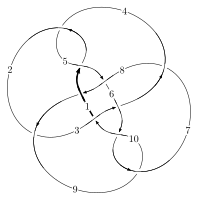
\includegraphics[width=112pt]{../../../GIT/diagram.site/Diagrams/png/204_10_120.png}\\
\ \ \ A knot diagram\footnotemark}&
\allowdisplaybreaks
\textbf{Linearized knot diagam} \\
\cline{2-2}
 &
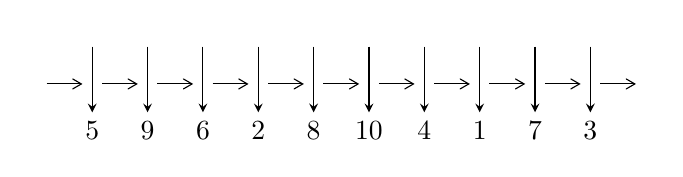
\begin{tikzpicture}[x=20pt, y=17pt]
	% nodes
	\node (C0) at (0, 0) {};
	\node (C1) at (1, 0) {};
	\node (C1U) at (1, +1) {};
	\node (C1D) at (1, -1) {5};

	\node (C2) at (2, 0) {};
	\node (C2U) at (2, +1) {};
	\node (C2D) at (2, -1) {9};

	\node (C3) at (3, 0) {};
	\node (C3U) at (3, +1) {};
	\node (C3D) at (3, -1) {6};

	\node (C4) at (4, 0) {};
	\node (C4U) at (4, +1) {};
	\node (C4D) at (4, -1) {2};

	\node (C5) at (5, 0) {};
	\node (C5U) at (5, +1) {};
	\node (C5D) at (5, -1) {8};

	\node (C6) at (6, 0) {};
	\node (C6U) at (6, +1) {};
	\node (C6D) at (6, -1) {10};

	\node (C7) at (7, 0) {};
	\node (C7U) at (7, +1) {};
	\node (C7D) at (7, -1) {4};

	\node (C8) at (8, 0) {};
	\node (C8U) at (8, +1) {};
	\node (C8D) at (8, -1) {1};

	\node (C9) at (9, 0) {};
	\node (C9U) at (9, +1) {};
	\node (C9D) at (9, -1) {7};

	\node (C10) at (10, 0) {};
	\node (C10U) at (10, +1) {};
	\node (C10D) at (10, -1) {3};
	\node (C11) at (11, 0) {};

	% arrows
	\draw[->,>={angle 60}]
	(C0) edge (C1) (C1) edge (C2) (C2) edge (C3) (C3) edge (C4) (C4) edge (C5) (C5) edge (C6) (C6) edge (C7) (C7) edge (C8) (C8) edge (C9) (C9) edge (C10) (C10) edge (C11) ;	\draw[->,>=stealth]
	(C1U) edge (C1D) (C2U) edge (C2D) (C3U) edge (C3D) (C4U) edge (C4D) (C5U) edge (C5D) (C6U) edge (C6D) (C7U) edge (C7D) (C8U) edge (C8D) (C9U) edge (C9D) (C10U) edge (C10D) ;
	\end{tikzpicture} \\
\hhline{~~} \\& 
\textbf{Solving Sequence} \\ \cline{2-2} 
 &
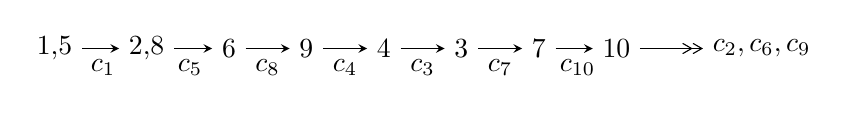
\begin{tikzpicture}[x=28pt, y=7pt]
	% node
	\node (A0) at (-1/8, 0) {1,5};
	\node (A1) at (17/16, 0) {2,8};
	\node (A2) at (17/8, 0) {6};
	\node (A3) at (25/8, 0) {9};
	\node (A4) at (33/8, 0) {4};
	\node (A5) at (41/8, 0) {3};
	\node (A6) at (49/8, 0) {7};
	\node (A7) at (57/8, 0) {10};
	\node (C1) at (1/2, -1) {$c_{1}$};
	\node (C2) at (13/8, -1) {$c_{5}$};
	\node (C3) at (21/8, -1) {$c_{8}$};
	\node (C4) at (29/8, -1) {$c_{4}$};
	\node (C5) at (37/8, -1) {$c_{3}$};
	\node (C6) at (45/8, -1) {$c_{7}$};
	\node (C7) at (53/8, -1) {$c_{10}$};
	\node (A8) at (9, 0) {$c_{2},c_{6},c_{9}$};

	% edge
	\draw[->,>=stealth]	
	(A0) edge (A1) (A1) edge (A2) (A2) edge (A3) (A3) edge (A4) (A4) edge (A5) (A5) edge (A6) (A6) edge (A7) ;
	\draw[->>,>={angle 60}]	
	(A7) edge (A8);
\end{tikzpicture} \\ 

\end{tabular} \\

\footnotetext{
The image of knot diagram is generated by the software ``\textbf{Draw programme}" developed by Andrew Bartholomew(\url{http://www.layer8.co.uk/maths/draw/index.htm\#Running-draw}), where we modified some parts for our purpose(\url{https://github.com/CATsTAILs/LinksPainter}).
}\phantom \\ \newline 
\centering \textbf{Ideals for irreducible components\footnotemark of $X_{\text{par}}$} 
 
\begin{align*}
I^u_{1}&=\langle 
- u^6- u^5-2 u^4- u^3- u^2+b- u+1,\\
\phantom{I^u_{1}}&\phantom{= \langle  }- u^{10}-3 u^9-8 u^8-13 u^7-19 u^6-20 u^5-19 u^4-13 u^3-7 u^2+2 a-2 u+2,\\
\phantom{I^u_{1}}&\phantom{= \langle  }u^{11}+3 u^{10}+8 u^9+13 u^8+19 u^7+22 u^6+21 u^5+17 u^4+9 u^3+4 u^2-2\rangle \\
I^u_{2}&=\langle 
- u^{17}-7 u^{16}+\cdots+b-13,\;-13 u^{17}-60 u^{16}+\cdots+5 a+4,\;u^{18}+5 u^{17}+\cdots+27 u+5\rangle \\
I^u_{3}&=\langle 
-3 u^{11}+11 u^{10}-29 u^9+50 u^8-66 u^7+71 u^6-59 u^5+43 u^4-22 u^3- a u+7 u^2+b-4 u,\\
\phantom{I^u_{3}}&\phantom{= \langle  }3 u^{10} a+u^{11}+\cdots+4 a-4,\;u^{12}-3 u^{11}+8 u^{10}-13 u^9+18 u^8-21 u^7+19 u^6-17 u^5+10 u^4-6 u^3+4 u^2+1\rangle \\
I^u_{4}&=\langle 
- a u+u^2+b- u+1,\;- u^2 a+a^2+u^2- a+1,\;u^3- u^2+2 u-1\rangle \\
I^u_{5}&=\langle 
u^2+b- u+1,\;u^2+a+1,\;u^3- u^2+2 u-1\rangle \\
I^u_{6}&=\langle 
u^6-4 u^5+8 u^4-11 u^3+9 u^2+b-5 u+3,\;-3 u^7+12 u^6-25 u^5+34 u^4-29 u^3+17 u^2+2 a-9 u+2,\\
\phantom{I^u_{6}}&\phantom{= \langle  }u^8-4 u^7+9 u^6-14 u^5+15 u^4-13 u^3+9 u^2-4 u+2\rangle \\
I^u_{7}&=\langle 
- a u+b+u-1,\;a^2- a u-1,\;u^2- u+1\rangle \\
\\
\end{align*}
\raggedright * 7 irreducible components of $\dim_{\mathbb{C}}=0$, with total 74 representations.\\
\footnotetext{All coefficients of polynomials are rational numbers. But the coefficients are sometimes approximated in decimal forms when there is not enough margin.}
\newpage
\renewcommand{\arraystretch}{1}
\centering \section*{I. $I^u_{1}= \langle - u^6- u^5-2 u^4- u^3- u^2+b- u+1,\;- u^{10}-3 u^9+\cdots+2 a+2,\;u^{11}+3 u^{10}+\cdots+4 u^2-2 \rangle$}
\flushleft \textbf{(i) Arc colorings}\\
\begin{tabular}{m{7pt} m{180pt} m{7pt} m{180pt} }
\flushright $a_{1}=$&$\begin{pmatrix}1\\0\end{pmatrix}$ \\
\flushright $a_{5}=$&$\begin{pmatrix}0\\u\end{pmatrix}$ \\
\flushright $a_{2}=$&$\begin{pmatrix}1\\u^2\end{pmatrix}$ \\
\flushright $a_{8}=$&$\begin{pmatrix}\frac{1}{2} u^{10}+\frac{3}{2} u^9+\cdots+u-1\\u^6+u^5+2 u^4+u^3+u^2+u-1\end{pmatrix}$ \\
\flushright $a_{6}=$&$\begin{pmatrix}\frac{1}{2} u^{10}+\frac{3}{2} u^9+\cdots-\frac{1}{2} u^2- u\\u^9+2 u^8+5 u^7+6 u^6+8 u^5+7 u^4+5 u^3+3 u^2+u-1\end{pmatrix}$ \\
\flushright $a_{9}=$&$\begin{pmatrix}\frac{1}{2} u^{10}+\frac{3}{2} u^9+\cdots+\frac{11}{2} u^3+\frac{5}{2} u^2\\u^6+u^5+2 u^4+u^3+u^2+u-1\end{pmatrix}$ \\
\flushright $a_{4}=$&$\begin{pmatrix}u\\u^3+u\end{pmatrix}$ \\
\flushright $a_{3}=$&$\begin{pmatrix}-\frac{1}{2} u^{10}-\frac{3}{2} u^9+\cdots+u+1\\- u^6- u^5-2 u^4- u^3- u^2- u+1\end{pmatrix}$ \\
\flushright $a_{7}=$&$\begin{pmatrix}\frac{1}{2} u^{10}+\frac{5}{2} u^9+\cdots+\frac{7}{2} u^2-1\\- u^{10}-3 u^9-7 u^8-11 u^7-14 u^6-15 u^5-12 u^4-8 u^3-3 u^2+1\end{pmatrix}$ \\
\flushright $a_{10}=$&$\begin{pmatrix}-\frac{1}{2} u^{10}-\frac{1}{2} u^9+\cdots+u-1\\- u^9-2 u^8-5 u^7-6 u^6-8 u^5-7 u^4-5 u^3-3 u^2+1\end{pmatrix}$\\&\end{tabular}
\flushleft \textbf{(ii) Obstruction class $= -1$}\\~\\
\flushleft \textbf{(iii) Cusp Shapes $= -2 u^8-6 u^7-14 u^6-18 u^5-24 u^4-18 u^3-16 u^2-6 u-6$}\\~\\
\newpage\renewcommand{\arraystretch}{1}
\flushleft \textbf{(iv) u-Polynomials at the component}\newline \\
\begin{tabular}{m{50pt}|m{274pt}}
Crossings & \hspace{64pt}u-Polynomials at each crossing \\
\hline $$\begin{aligned}c_{1},c_{4},c_{6}\\c_{9}\end{aligned}$$&$\begin{aligned}
&u^{11}-3 u^{10}+8 u^9-13 u^8+19 u^7-22 u^6+21 u^5-17 u^4+9 u^3-4 u^2+2
\end{aligned}$\\
\hline $$\begin{aligned}c_{2},c_{7}\end{aligned}$$&$\begin{aligned}
&u^{11}+5 u^{10}+\cdots+10 u+4
\end{aligned}$\\
\hline $$\begin{aligned}c_{3},c_{5},c_{8}\\c_{10}\end{aligned}$$&$\begin{aligned}
&u^{11}+4 u^9+u^8+11 u^7+4 u^6+15 u^5+3 u^4+9 u^3- u^2+2 u+1
\end{aligned}$\\
\hline
\end{tabular}\\~\\
\newpage\renewcommand{\arraystretch}{1}
\flushleft \textbf{(v) Riley Polynomials at the component}\newline \\
\begin{tabular}{m{50pt}|m{274pt}}
Crossings & \hspace{64pt}Riley Polynomials at each crossing \\
\hline $$\begin{aligned}c_{1},c_{4},c_{6}\\c_{9}\end{aligned}$$&$\begin{aligned}
&y^{11}+7 y^{10}+\cdots+16 y-4
\end{aligned}$\\
\hline $$\begin{aligned}c_{2},c_{7}\end{aligned}$$&$\begin{aligned}
&y^{11}-5 y^{10}+\cdots+60 y-16
\end{aligned}$\\
\hline $$\begin{aligned}c_{3},c_{5},c_{8}\\c_{10}\end{aligned}$$&$\begin{aligned}
&y^{11}+8 y^{10}+\cdots+6 y-1
\end{aligned}$\\
\hline
\end{tabular}\\~\\
\newpage\flushleft \textbf{(vi) Complex Volumes and Cusp Shapes}
$$\begin{array}{c|c|c}  
\text{Solutions to }I^u_{1}& \I (\text{vol} + \sqrt{-1}CS) & \text{Cusp shape}\\
 \hline 
\begin{aligned}
u &= -0.955959 + 0.181916 I \\
a &= -0.517203 - 1.103780 I \\
b &= -0.695220 - 0.961079 I\end{aligned}
 & -0.51987 - 4.74721 I & -10.74299 + 5.17166 I \\ \hline\begin{aligned}
u &= -0.955959 - 0.181916 I \\
a &= -0.517203 + 1.103780 I \\
b &= -0.695220 + 0.961079 I\end{aligned}
 & -0.51987 + 4.74721 I & -10.74299 - 5.17166 I \\ \hline\begin{aligned}
u &= \phantom{-}0.104833 + 1.064770 I \\
a &= -1.051120 - 0.609326 I \\
b &= -0.538602 + 1.183080 I\end{aligned}
 & \phantom{-}5.39093 - 0.52336 I & -2.07555 - 0.88155 I \\ \hline\begin{aligned}
u &= \phantom{-}0.104833 - 1.064770 I \\
a &= -1.051120 + 0.609326 I \\
b &= -0.538602 - 1.183080 I\end{aligned}
 & \phantom{-}5.39093 + 0.52336 I & -2.07555 + 0.88155 I \\ \hline\begin{aligned}
u &= \phantom{-}0.375570 + 1.042270 I \\
a &= \phantom{-}0.289036 + 0.451507 I \\
b &= \phantom{-}0.362037 - 0.470824 I\end{aligned}
 & \phantom{-}2.05520 - 3.23878 I & -8.62571 + 3.68812 I \\ \hline\begin{aligned}
u &= \phantom{-}0.375570 - 1.042270 I \\
a &= \phantom{-}0.289036 - 0.451507 I \\
b &= \phantom{-}0.362037 + 0.470824 I\end{aligned}
 & \phantom{-}2.05520 + 3.23878 I & -8.62571 - 3.68812 I \\ \hline\begin{aligned}
u &= -0.641442 + 1.159660 I \\
a &= -0.736546 + 0.484569 I \\
b &= \phantom{-}0.089483 + 1.164960 I\end{aligned}
 & \phantom{-}6.47745 + 4.30838 I & -1.34168 - 3.93056 I \\ \hline\begin{aligned}
u &= -0.641442 - 1.159660 I \\
a &= -0.736546 - 0.484569 I \\
b &= \phantom{-}0.089483 - 1.164960 I\end{aligned}
 & \phantom{-}6.47745 - 4.30838 I & -1.34168 + 3.93056 I \\ \hline\begin{aligned}
u &= -0.58305 + 1.34141 I \\
a &= \phantom{-}1.128180 + 0.208445 I \\
b &= \phantom{-}0.93740 - 1.39182 I\end{aligned}
 & \phantom{-}6.7235 + 16.2714 I & -5.72276 - 8.85281 I \\ \hline\begin{aligned}
u &= -0.58305 - 1.34141 I \\
a &= \phantom{-}1.128180 - 0.208445 I \\
b &= \phantom{-}0.93740 + 1.39182 I\end{aligned}
 & \phantom{-}6.7235 - 16.2714 I & -5.72276 + 8.85281 I\\
 \hline 
 \end{array}$$\newpage$$\begin{array}{c|c|c}  
\text{Solutions to }I^u_{1}& \I (\text{vol} + \sqrt{-1}CS) & \text{Cusp shape}\\
 \hline 
\begin{aligned}
u &= \phantom{-}0.400093\phantom{ +0.000000I} \\
a &= \phantom{-}0.775290\phantom{ +0.000000I} \\
b &= -0.310188\phantom{ +0.000000I}\end{aligned}
 & -0.775978\phantom{ +0.000000I} & -12.9830\phantom{ +0.000000I}\\
 \hline 
 \end{array}$$\newpage\newpage\renewcommand{\arraystretch}{1}
\centering \section*{II. $I^u_{2}= \langle - u^{17}-7 u^{16}+\cdots+b-13,\;-13 u^{17}-60 u^{16}+\cdots+5 a+4,\;u^{18}+5 u^{17}+\cdots+27 u+5 \rangle$}
\flushleft \textbf{(i) Arc colorings}\\
\begin{tabular}{m{7pt} m{180pt} m{7pt} m{180pt} }
\flushright $a_{1}=$&$\begin{pmatrix}1\\0\end{pmatrix}$ \\
\flushright $a_{5}=$&$\begin{pmatrix}0\\u\end{pmatrix}$ \\
\flushright $a_{2}=$&$\begin{pmatrix}1\\u^2\end{pmatrix}$ \\
\flushright $a_{8}=$&$\begin{pmatrix}\frac{13}{5} u^{17}+12 u^{16}+\cdots+\frac{77}{5} u-\frac{4}{5}\\u^{17}+7 u^{16}+\cdots+71 u+13\end{pmatrix}$ \\
\flushright $a_{6}=$&$\begin{pmatrix}-\frac{11}{5} u^{17}-11 u^{16}+\cdots-\frac{229}{5} u-\frac{42}{5}\\-3 u^{15}-13 u^{14}+\cdots-50 u-11\end{pmatrix}$ \\
\flushright $a_{9}=$&$\begin{pmatrix}\frac{8}{5} u^{17}+5 u^{16}+\cdots-\frac{278}{5} u-\frac{69}{5}\\u^{17}+7 u^{16}+\cdots+71 u+13\end{pmatrix}$ \\
\flushright $a_{4}=$&$\begin{pmatrix}u\\u^3+u\end{pmatrix}$ \\
\flushright $a_{3}=$&$\begin{pmatrix}\frac{4}{5} u^{17}+8 u^{16}+\cdots+\frac{391}{5} u+\frac{73}{5}\\-3 u^{17}-16 u^{16}+\cdots-62 u-11\end{pmatrix}$ \\
\flushright $a_{7}=$&$\begin{pmatrix}\frac{13}{5} u^{17}+13 u^{16}+\cdots+\frac{67}{5} u-\frac{4}{5}\\u^{16}+5 u^{15}+\cdots+42 u+8\end{pmatrix}$ \\
\flushright $a_{10}=$&$\begin{pmatrix}\frac{9}{5} u^{17}+6 u^{16}+\cdots-\frac{189}{5} u-\frac{32}{5}\\- u^{17}-4 u^{16}+\cdots+16 u+4\end{pmatrix}$\\&\end{tabular}
\flushleft \textbf{(ii) Obstruction class $= -1$}\\~\\
\flushleft \textbf{(iii) Cusp Shapes $= 26 u^{17}+130 u^{16}+415 u^{15}+871 u^{14}+1236 u^{13}+1002 u^{12}-275 u^{11}-2187 u^{10}-3562 u^9-3091 u^8-569 u^7+2567 u^6+4603 u^5+4614 u^4+3181 u^3+1560 u^2+486 u+63$}\\~\\
\newpage\renewcommand{\arraystretch}{1}
\flushleft \textbf{(iv) u-Polynomials at the component}\newline \\
\begin{tabular}{m{50pt}|m{274pt}}
Crossings & \hspace{64pt}u-Polynomials at each crossing \\
\hline $$\begin{aligned}c_{1},c_{4},c_{6}\\c_{9}\end{aligned}$$&$\begin{aligned}
&u^{18}-5 u^{17}+\cdots-27 u+5
\end{aligned}$\\
\hline $$\begin{aligned}c_{2},c_{7}\end{aligned}$$&$\begin{aligned}
&(u^9-2 u^8+4 u^7-5 u^6+7 u^5-5 u^4+3 u^3-2 u^2+u-1)^2
\end{aligned}$\\
\hline $$\begin{aligned}c_{3},c_{5},c_{8}\\c_{10}\end{aligned}$$&$\begin{aligned}
&u^{18}- u^{17}+\cdots+3 u+1
\end{aligned}$\\
\hline
\end{tabular}\\~\\
\newpage\renewcommand{\arraystretch}{1}
\flushleft \textbf{(v) Riley Polynomials at the component}\newline \\
\begin{tabular}{m{50pt}|m{274pt}}
Crossings & \hspace{64pt}Riley Polynomials at each crossing \\
\hline $$\begin{aligned}c_{1},c_{4},c_{6}\\c_{9}\end{aligned}$$&$\begin{aligned}
&y^{18}+9 y^{17}+\cdots+61 y+25
\end{aligned}$\\
\hline $$\begin{aligned}c_{2},c_{7}\end{aligned}$$&$\begin{aligned}
&(y^9+4 y^8+10 y^7+17 y^6+17 y^5+y^4-7 y^3-8 y^2-3 y-1)^2
\end{aligned}$\\
\hline $$\begin{aligned}c_{3},c_{5},c_{8}\\c_{10}\end{aligned}$$&$\begin{aligned}
&y^{18}+9 y^{17}+\cdots+43 y+1
\end{aligned}$\\
\hline
\end{tabular}\\~\\
\newpage\flushleft \textbf{(vi) Complex Volumes and Cusp Shapes}
$$\begin{array}{c|c|c}  
\text{Solutions to }I^u_{2}& \I (\text{vol} + \sqrt{-1}CS) & \text{Cusp shape}\\
 \hline 
\begin{aligned}
u &= -0.198527 + 0.827118 I \\
a &= -0.81586 - 1.28949 I \\
b &= -1.228530 + 0.418813 I\end{aligned}
 & -1.04793 + 1.11007 I & -17.5535 - 4.7867 I \\ \hline\begin{aligned}
u &= -0.198527 - 0.827118 I \\
a &= -0.81586 + 1.28949 I \\
b &= -1.228530 - 0.418813 I\end{aligned}
 & -1.04793 - 1.11007 I & -17.5535 + 4.7867 I \\ \hline\begin{aligned}
u &= -0.079308 + 0.836177 I \\
a &= \phantom{-}1.38823 + 0.30834 I \\
b &= \phantom{-}0.367922 - 1.136350 I\end{aligned}
 & \phantom{-}4.23983\phantom{ +0.000000I} & -2.85705 + 0. I\phantom{ +0.000000I} \\ \hline\begin{aligned}
u &= -0.079308 - 0.836177 I \\
a &= \phantom{-}1.38823 - 0.30834 I \\
b &= \phantom{-}0.367922 + 1.136350 I\end{aligned}
 & \phantom{-}4.23983\phantom{ +0.000000I} & -2.85705 + 0. I\phantom{ +0.000000I} \\ \hline\begin{aligned}
u &= -1.156420 + 0.102576 I \\
a &= \phantom{-}0.521985 + 0.890705 I \\
b &= \phantom{-}0.694998 + 0.976484 I\end{aligned}
 & \phantom{-}2.81259 - 10.16840 I & -7.74812 + 7.64867 I \\ \hline\begin{aligned}
u &= -1.156420 - 0.102576 I \\
a &= \phantom{-}0.521985 - 0.890705 I \\
b &= \phantom{-}0.694998 - 0.976484 I\end{aligned}
 & \phantom{-}2.81259 + 10.16840 I & -7.74812 - 7.64867 I \\ \hline\begin{aligned}
u &= \phantom{-}1.160130 + 0.229157 I \\
a &= \phantom{-}0.035605 - 0.158300 I \\
b &= -0.077582 + 0.175489 I\end{aligned}
 & -1.04793 - 1.11007 I & -17.5535 + 4.7867 I \\ \hline\begin{aligned}
u &= \phantom{-}1.160130 - 0.229157 I \\
a &= \phantom{-}0.035605 + 0.158300 I \\
b &= -0.077582 - 0.175489 I\end{aligned}
 & -1.04793 + 1.11007 I & -17.5535 - 4.7867 I \\ \hline\begin{aligned}
u &= -0.311796 + 1.205210 I \\
a &= \phantom{-}0.814403 - 0.074315 I \\
b &= \phantom{-}0.164362 - 1.004700 I\end{aligned}
 & \phantom{-}4.26456 - 0.69984 I & -4.65022 + 1.89978 I \\ \hline\begin{aligned}
u &= -0.311796 - 1.205210 I \\
a &= \phantom{-}0.814403 + 0.074315 I \\
b &= \phantom{-}0.164362 + 1.004700 I\end{aligned}
 & \phantom{-}4.26456 + 0.69984 I & -4.65022 - 1.89978 I\\
 \hline 
 \end{array}$$\newpage$$\begin{array}{c|c|c}  
\text{Solutions to }I^u_{2}& \I (\text{vol} + \sqrt{-1}CS) & \text{Cusp shape}\\
 \hline 
\begin{aligned}
u &= -0.369880 + 1.229190 I \\
a &= \phantom{-}1.216830 + 0.459753 I \\
b &= \phantom{-}1.01520 - 1.32566 I\end{aligned}
 & \phantom{-}8.30021 + 4.38855 I & -1.11965 - 3.68700 I \\ \hline\begin{aligned}
u &= -0.369880 - 1.229190 I \\
a &= \phantom{-}1.216830 - 0.459753 I \\
b &= \phantom{-}1.01520 + 1.32566 I\end{aligned}
 & \phantom{-}8.30021 - 4.38855 I & -1.11965 + 3.68700 I \\ \hline\begin{aligned}
u &= -0.642487 + 0.199869 I \\
a &= \phantom{-}1.21195 - 1.14348 I \\
b &= \phantom{-}0.550112 - 0.976904 I\end{aligned}
 & \phantom{-}4.26456 + 0.69984 I & -4.65022 - 1.89978 I \\ \hline\begin{aligned}
u &= -0.642487 - 0.199869 I \\
a &= \phantom{-}1.21195 + 1.14348 I \\
b &= \phantom{-}0.550112 + 0.976904 I\end{aligned}
 & \phantom{-}4.26456 - 0.69984 I & -4.65022 + 1.89978 I \\ \hline\begin{aligned}
u &= -0.545158 + 1.253180 I \\
a &= -1.229130 - 0.230487 I \\
b &= -0.95891 + 1.41466 I\end{aligned}
 & \phantom{-}2.81259 + 10.16840 I & -7.74812 - 7.64867 I \\ \hline\begin{aligned}
u &= -0.545158 - 1.253180 I \\
a &= -1.229130 + 0.230487 I \\
b &= -0.95891 - 1.41466 I\end{aligned}
 & \phantom{-}2.81259 - 10.16840 I & -7.74812 + 7.64867 I \\ \hline\begin{aligned}
u &= -0.35655 + 1.50992 I \\
a &= -0.544015 + 0.110198 I \\
b &= -0.027580 + 0.860709 I\end{aligned}
 & \phantom{-}8.30021 - 4.38855 I & -1.11965 + 3.68700 I \\ \hline\begin{aligned}
u &= -0.35655 - 1.50992 I \\
a &= -0.544015 - 0.110198 I \\
b &= -0.027580 - 0.860709 I\end{aligned}
 & \phantom{-}8.30021 + 4.38855 I & -1.11965 - 3.68700 I\\
 \hline 
 \end{array}$$\newpage\newpage\renewcommand{\arraystretch}{1}
\centering \section*{III. $I^u_{3}= \langle -3 u^{11}+11 u^{10}+\cdots+b-4 u,\;3 u^{10} a+u^{11}+\cdots+4 a-4,\;u^{12}-3 u^{11}+\cdots+4 u^2+1 \rangle$}
\flushleft \textbf{(i) Arc colorings}\\
\begin{tabular}{m{7pt} m{180pt} m{7pt} m{180pt} }
\flushright $a_{1}=$&$\begin{pmatrix}1\\0\end{pmatrix}$ \\
\flushright $a_{5}=$&$\begin{pmatrix}0\\u\end{pmatrix}$ \\
\flushright $a_{2}=$&$\begin{pmatrix}1\\u^2\end{pmatrix}$ \\
\flushright $a_{8}=$&$\begin{pmatrix}a\\3 u^{11}-11 u^{10}+\cdots+a u+4 u\end{pmatrix}$ \\
\flushright $a_{6}=$&$\begin{pmatrix}3 u^{11} a- u^{11}+\cdots-4 u-1\\1\end{pmatrix}$ \\
\flushright $a_{9}=$&$\begin{pmatrix}-3 u^{11}+11 u^{10}+\cdots+a-4 u\\3 u^{11}-11 u^{10}+\cdots+a u+4 u\end{pmatrix}$ \\
\flushright $a_{4}=$&$\begin{pmatrix}u\\u^3+u\end{pmatrix}$ \\
\flushright $a_{3}=$&$\begin{pmatrix}-2 u^{11} a+u^{11}+\cdots- a+2\\- u^{10} a+4 u^9 a+\cdots-2 a+1\end{pmatrix}$ \\
\flushright $a_{7}=$&$\begin{pmatrix}- u^{11}+5 u^{10}+\cdots+a+2\\2 u^{11}-7 u^{10}+\cdots+a u+2 u\end{pmatrix}$ \\
\flushright $a_{10}=$&$\begin{pmatrix}- u^{10} a- u^{11}+\cdots+a-2\\- u^7 a+u^6 a+\cdots+a+1\end{pmatrix}$\\&\end{tabular}
\flushleft \textbf{(ii) Obstruction class $= -1$}\\~\\
\flushleft \textbf{(iii) Cusp Shapes $= 4 u^{11}-16 u^{10}+44 u^9-80 u^8+112 u^7-124 u^6+116 u^5-92 u^4+60 u^3-28 u^2+8 u-18$}\\~\\
\newpage\renewcommand{\arraystretch}{1}
\flushleft \textbf{(iv) u-Polynomials at the component}\newline \\
\begin{tabular}{m{50pt}|m{274pt}}
Crossings & \hspace{64pt}u-Polynomials at each crossing \\
\hline $$\begin{aligned}c_{1},c_{4},c_{6}\\c_{9}\end{aligned}$$&$\begin{aligned}
&(u^{12}+3 u^{11}+\cdots+4 u^2+1)^{2}
\end{aligned}$\\
\hline $$\begin{aligned}c_{2},c_{7}\end{aligned}$$&$\begin{aligned}
&(u^{12}+u^{10}-6 u^9+10 u^8-2 u^7+2 u^6-2 u^4+2 u^2+1)^2
\end{aligned}$\\
\hline $$\begin{aligned}c_{3},c_{5},c_{8}\\c_{10}\end{aligned}$$&$\begin{aligned}
&u^{24}-3 u^{23}+\cdots-4 u^2+1
\end{aligned}$\\
\hline
\end{tabular}\\~\\
\newpage\renewcommand{\arraystretch}{1}
\flushleft \textbf{(v) Riley Polynomials at the component}\newline \\
\begin{tabular}{m{50pt}|m{274pt}}
Crossings & \hspace{64pt}Riley Polynomials at each crossing \\
\hline $$\begin{aligned}c_{1},c_{4},c_{6}\\c_{9}\end{aligned}$$&$\begin{aligned}
&(y^{12}+7 y^{11}+\cdots+8 y+1)^{2}
\end{aligned}$\\
\hline $$\begin{aligned}c_{2},c_{7}\end{aligned}$$&$\begin{aligned}
&(y^{12}+2 y^{11}+\cdots+4 y+1)^{2}
\end{aligned}$\\
\hline $$\begin{aligned}c_{3},c_{5},c_{8}\\c_{10}\end{aligned}$$&$\begin{aligned}
&y^{24}-11 y^{23}+\cdots-8 y+1
\end{aligned}$\\
\hline
\end{tabular}\\~\\
\newpage\flushleft \textbf{(vi) Complex Volumes and Cusp Shapes}
$$\begin{array}{c|c|c}  
\text{Solutions to }I^u_{3}& \I (\text{vol} + \sqrt{-1}CS) & \text{Cusp shape}\\
 \hline 
\begin{aligned}
u &= -0.234552 + 1.002020 I \\
a &= \phantom{-}0.647681 + 0.298955 I \\
b &= \phantom{-}2.11054 + 0.48664 I\end{aligned}
 & \phantom{-}3.72285 + 6.96551 I & -5.97171 - 10.57440 I \\ \hline\begin{aligned}
u &= -0.234552 + 1.002020 I \\
a &= \phantom{-}0.00700 + 2.10465 I \\
b &= \phantom{-}0.451474 - 0.578868 I\end{aligned}
 & \phantom{-}3.72285 + 6.96551 I & -5.97171 - 10.57440 I \\ \hline\begin{aligned}
u &= -0.234552 - 1.002020 I \\
a &= \phantom{-}0.647681 - 0.298955 I \\
b &= \phantom{-}2.11054 - 0.48664 I\end{aligned}
 & \phantom{-}3.72285 - 6.96551 I & -5.97171 + 10.57440 I \\ \hline\begin{aligned}
u &= -0.234552 - 1.002020 I \\
a &= \phantom{-}0.00700 - 2.10465 I \\
b &= \phantom{-}0.451474 + 0.578868 I\end{aligned}
 & \phantom{-}3.72285 - 6.96551 I & -5.97171 + 10.57440 I \\ \hline\begin{aligned}
u &= \phantom{-}1.090290 + 0.140460 I \\
a &= -0.240626 - 0.291610 I \\
b &= -0.401743 + 0.003834 I\end{aligned}
 & -1.05784 - 1.08263 I & -14.2815 + 5.6276 I \\ \hline\begin{aligned}
u &= \phantom{-}1.090290 + 0.140460 I \\
a &= \phantom{-}0.362012 - 0.050153 I \\
b &= \phantom{-}0.221393 + 0.351739 I\end{aligned}
 & -1.05784 - 1.08263 I & -14.2815 + 5.6276 I \\ \hline\begin{aligned}
u &= \phantom{-}1.090290 - 0.140460 I \\
a &= -0.240626 + 0.291610 I \\
b &= -0.401743 - 0.003834 I\end{aligned}
 & -1.05784 + 1.08263 I & -14.2815 - 5.6276 I \\ \hline\begin{aligned}
u &= \phantom{-}1.090290 - 0.140460 I \\
a &= \phantom{-}0.362012 + 0.050153 I \\
b &= \phantom{-}0.221393 - 0.351739 I\end{aligned}
 & -1.05784 + 1.08263 I & -14.2815 - 5.6276 I \\ \hline\begin{aligned}
u &= -0.185688 + 0.817666 I \\
a &= -0.762192 - 0.903819 I \\
b &= -1.44128 + 0.18321 I\end{aligned}
 & -1.05784 + 1.08263 I & -14.2815 - 5.6276 I \\ \hline\begin{aligned}
u &= -0.185688 + 0.817666 I \\
a &= -0.59374 - 1.62783 I \\
b &= -0.880553 + 0.455390 I\end{aligned}
 & -1.05784 + 1.08263 I & -14.2815 - 5.6276 I\\
 \hline 
 \end{array}$$\newpage$$\begin{array}{c|c|c}  
\text{Solutions to }I^u_{3}& \I (\text{vol} + \sqrt{-1}CS) & \text{Cusp shape}\\
 \hline 
\begin{aligned}
u &= -0.185688 - 0.817666 I \\
a &= -0.762192 + 0.903819 I \\
b &= -1.44128 - 0.18321 I\end{aligned}
 & -1.05784 - 1.08263 I & -14.2815 + 5.6276 I \\ \hline\begin{aligned}
u &= -0.185688 - 0.817666 I \\
a &= -0.59374 + 1.62783 I \\
b &= -0.880553 - 0.455390 I\end{aligned}
 & -1.05784 - 1.08263 I & -14.2815 + 5.6276 I \\ \hline\begin{aligned}
u &= \phantom{-}0.529049 + 1.245360 I \\
a &= \phantom{-}0.970902 - 0.051810 I \\
b &= \phantom{-}0.692981 + 0.737589 I\end{aligned}
 & \phantom{-}2.26979 - 4.55813 I & -9.74676 + 1.77049 I \\ \hline\begin{aligned}
u &= \phantom{-}0.529049 + 1.245360 I \\
a &= -0.701975 + 0.258240 I \\
b &= -0.578176 - 1.181710 I\end{aligned}
 & \phantom{-}2.26979 - 4.55813 I & -9.74676 + 1.77049 I \\ \hline\begin{aligned}
u &= \phantom{-}0.529049 - 1.245360 I \\
a &= \phantom{-}0.970902 + 0.051810 I \\
b &= \phantom{-}0.692981 - 0.737589 I\end{aligned}
 & \phantom{-}2.26979 + 4.55813 I & -9.74676 - 1.77049 I \\ \hline\begin{aligned}
u &= \phantom{-}0.529049 - 1.245360 I \\
a &= -0.701975 - 0.258240 I \\
b &= -0.578176 + 1.181710 I\end{aligned}
 & \phantom{-}2.26979 + 4.55813 I & -9.74676 - 1.77049 I \\ \hline\begin{aligned}
u &= -0.251512 + 0.449740 I \\
a &= \phantom{-}0.04323 + 2.16308 I \\
b &= \phantom{-}0.800711 - 0.884208 I\end{aligned}
 & \phantom{-}2.26979 - 4.55813 I & -9.74676 + 1.77049 I \\ \hline\begin{aligned}
u &= -0.251512 + 0.449740 I \\
a &= \phantom{-}2.25611 + 0.51868 I \\
b &= \phantom{-}0.983696 + 0.524600 I\end{aligned}
 & \phantom{-}2.26979 - 4.55813 I & -9.74676 + 1.77049 I \\ \hline\begin{aligned}
u &= -0.251512 - 0.449740 I \\
a &= \phantom{-}0.04323 - 2.16308 I \\
b &= \phantom{-}0.800711 + 0.884208 I\end{aligned}
 & \phantom{-}2.26979 + 4.55813 I & -9.74676 - 1.77049 I \\ \hline\begin{aligned}
u &= -0.251512 - 0.449740 I \\
a &= \phantom{-}2.25611 - 0.51868 I \\
b &= \phantom{-}0.983696 - 0.524600 I\end{aligned}
 & \phantom{-}2.26979 + 4.55813 I & -9.74676 - 1.77049 I\\
 \hline 
 \end{array}$$\newpage$$\begin{array}{c|c|c}  
\text{Solutions to }I^u_{3}& \I (\text{vol} + \sqrt{-1}CS) & \text{Cusp shape}\\
 \hline 
\begin{aligned}
u &= \phantom{-}0.55241 + 1.40748 I \\
a &= \phantom{-}0.767735 - 0.370784 I \\
b &= \phantom{-}0.486934 + 1.037080 I\end{aligned}
 & \phantom{-}3.72285 - 6.96551 I & -5.97171 + 10.57440 I \\ \hline\begin{aligned}
u &= \phantom{-}0.55241 + 1.40748 I \\
a &= -0.756136 + 0.049190 I \\
b &= -0.945979 - 0.875748 I\end{aligned}
 & \phantom{-}3.72285 - 6.96551 I & -5.97171 + 10.57440 I \\ \hline\begin{aligned}
u &= \phantom{-}0.55241 - 1.40748 I \\
a &= \phantom{-}0.767735 + 0.370784 I \\
b &= \phantom{-}0.486934 - 1.037080 I\end{aligned}
 & \phantom{-}3.72285 + 6.96551 I & -5.97171 - 10.57440 I \\ \hline\begin{aligned}
u &= \phantom{-}0.55241 - 1.40748 I \\
a &= -0.756136 - 0.049190 I \\
b &= -0.945979 + 0.875748 I\end{aligned}
 & \phantom{-}3.72285 + 6.96551 I & -5.97171 - 10.57440 I\\
 \hline 
 \end{array}$$\newpage\newpage\renewcommand{\arraystretch}{1}
\centering \section*{IV. $I^u_{4}= \langle - a u+u^2+b- u+1,\;- u^2 a+a^2+u^2- a+1,\;u^3- u^2+2 u-1 \rangle$}
\flushleft \textbf{(i) Arc colorings}\\
\begin{tabular}{m{7pt} m{180pt} m{7pt} m{180pt} }
\flushright $a_{1}=$&$\begin{pmatrix}1\\0\end{pmatrix}$ \\
\flushright $a_{5}=$&$\begin{pmatrix}0\\u\end{pmatrix}$ \\
\flushright $a_{2}=$&$\begin{pmatrix}1\\u^2\end{pmatrix}$ \\
\flushright $a_{8}=$&$\begin{pmatrix}a\\a u- u^2+u-1\end{pmatrix}$ \\
\flushright $a_{6}=$&$\begin{pmatrix}- u^2 a+a u+u^2- a- u+1\\1\end{pmatrix}$ \\
\flushright $a_{9}=$&$\begin{pmatrix}- a u+u^2+a- u+1\\a u- u^2+u-1\end{pmatrix}$ \\
\flushright $a_{4}=$&$\begin{pmatrix}u\\u^2- u+1\end{pmatrix}$ \\
\flushright $a_{3}=$&$\begin{pmatrix}2 a u- a\\- a u+u^2- u+1\end{pmatrix}$ \\
\flushright $a_{7}=$&$\begin{pmatrix}u^2 a- a u+u^2+a- u\\- u^2 a+a u-2 u^2+u-1\end{pmatrix}$ \\
\flushright $a_{10}=$&$\begin{pmatrix}u^2+u\\- a u+a-2 u+1\end{pmatrix}$\\&\end{tabular}
\flushleft \textbf{(ii) Obstruction class $= -1$}\\~\\
\flushleft \textbf{(iii) Cusp Shapes $= -8 u^2+8 u-14$}\\~\\
\newpage\renewcommand{\arraystretch}{1}
\flushleft \textbf{(iv) u-Polynomials at the component}\newline \\
\begin{tabular}{m{50pt}|m{274pt}}
Crossings & \hspace{64pt}u-Polynomials at each crossing \\
\hline $$\begin{aligned}c_{1},c_{4},c_{6}\\c_{9}\end{aligned}$$&$\begin{aligned}
&(u^3+u^2+2 u+1)^2
\end{aligned}$\\
\hline $$\begin{aligned}c_{2},c_{7}\end{aligned}$$&$\begin{aligned}
&u^6+5 u^5+16 u^4+28 u^3+30 u^2+18 u+5
\end{aligned}$\\
\hline $$\begin{aligned}c_{3},c_{5},c_{8}\\c_{10}\end{aligned}$$&$\begin{aligned}
&u^6- u^5+2 u^4+2 u^3+4 u^2+2 u+1
\end{aligned}$\\
\hline
\end{tabular}\\~\\
\newpage\renewcommand{\arraystretch}{1}
\flushleft \textbf{(v) Riley Polynomials at the component}\newline \\
\begin{tabular}{m{50pt}|m{274pt}}
Crossings & \hspace{64pt}Riley Polynomials at each crossing \\
\hline $$\begin{aligned}c_{1},c_{4},c_{6}\\c_{9}\end{aligned}$$&$\begin{aligned}
&(y^3+3 y^2+2 y-1)^2
\end{aligned}$\\
\hline $$\begin{aligned}c_{2},c_{7}\end{aligned}$$&$\begin{aligned}
&y^6+7 y^5+36 y^4+6 y^3+52 y^2-24 y+25
\end{aligned}$\\
\hline $$\begin{aligned}c_{3},c_{5},c_{8}\\c_{10}\end{aligned}$$&$\begin{aligned}
&y^6+3 y^5+16 y^4+18 y^3+12 y^2+4 y+1
\end{aligned}$\\
\hline
\end{tabular}\\~\\
\newpage\flushleft \textbf{(vi) Complex Volumes and Cusp Shapes}
$$\begin{array}{c|c|c}  
\text{Solutions to }I^u_{4}& \I (\text{vol} + \sqrt{-1}CS) & \text{Cusp shape}\\
 \hline 
\begin{aligned}
u &= \phantom{-}0.215080 + 1.307140 I \\
a &= \phantom{-}0.594305 - 0.123240 I \\
b &= \phantom{-}1.16635 + 1.49520 I\end{aligned}
 & \phantom{-}7.69319 - 5.65624 I & \phantom{-}1.01951 + 5.95889 I \\ \hline\begin{aligned}
u &= \phantom{-}0.215080 + 1.307140 I \\
a &= -1.25666 + 0.68552 I \\
b &= -0.288915 - 0.750335 I\end{aligned}
 & \phantom{-}7.69319 - 5.65624 I & \phantom{-}1.01951 + 5.95889 I \\ \hline\begin{aligned}
u &= \phantom{-}0.215080 - 1.307140 I \\
a &= \phantom{-}0.594305 + 0.123240 I \\
b &= \phantom{-}1.16635 - 1.49520 I\end{aligned}
 & \phantom{-}7.69319 + 5.65624 I & \phantom{-}1.01951 - 5.95889 I \\ \hline\begin{aligned}
u &= \phantom{-}0.215080 - 1.307140 I \\
a &= -1.25666 - 0.68552 I \\
b &= -0.288915 + 0.750335 I\end{aligned}
 & \phantom{-}7.69319 + 5.65624 I & \phantom{-}1.01951 - 5.95889 I \\ \hline\begin{aligned}
u &= \phantom{-}0.569840\phantom{ +0.000000I} \\
a &= \phantom{-}0.662359 + 0.941275 I \\
b &= -0.377439 + 0.536376 I\end{aligned}
 & -0.581975\phantom{ +0.000000I} & -12.0390\phantom{ +0.000000I} \\ \hline\begin{aligned}
u &= \phantom{-}0.569840\phantom{ +0.000000I} \\
a &= \phantom{-}0.662359 - 0.941275 I \\
b &= -0.377439 - 0.536376 I\end{aligned}
 & -0.581975\phantom{ +0.000000I} & -12.0390\phantom{ +0.000000I}\\
 \hline 
 \end{array}$$\newpage\newpage\renewcommand{\arraystretch}{1}
\centering \section*{V. $I^u_{5}= \langle u^2+b- u+1,\;u^2+a+1,\;u^3- u^2+2 u-1 \rangle$}
\flushleft \textbf{(i) Arc colorings}\\
\begin{tabular}{m{7pt} m{180pt} m{7pt} m{180pt} }
\flushright $a_{1}=$&$\begin{pmatrix}1\\0\end{pmatrix}$ \\
\flushright $a_{5}=$&$\begin{pmatrix}0\\u\end{pmatrix}$ \\
\flushright $a_{2}=$&$\begin{pmatrix}1\\u^2\end{pmatrix}$ \\
\flushright $a_{8}=$&$\begin{pmatrix}- u^2-1\\- u^2+u-1\end{pmatrix}$ \\
\flushright $a_{6}=$&$\begin{pmatrix}-1\\0\end{pmatrix}$ \\
\flushright $a_{9}=$&$\begin{pmatrix}- u\\- u^2+u-1\end{pmatrix}$ \\
\flushright $a_{4}=$&$\begin{pmatrix}u\\u^2- u+1\end{pmatrix}$ \\
\flushright $a_{3}=$&$\begin{pmatrix}u^2+1\\u^2- u+1\end{pmatrix}$ \\
\flushright $a_{7}=$&$\begin{pmatrix}-1\\- u^2\end{pmatrix}$ \\
\flushright $a_{10}=$&$\begin{pmatrix}0\\- u\end{pmatrix}$\\&\end{tabular}
\flushleft \textbf{(ii) Obstruction class $= 1$}\\~\\
\flushleft \textbf{(iii) Cusp Shapes $= -8 u^2+8 u-20$}\\~\\
\newpage\renewcommand{\arraystretch}{1}
\flushleft \textbf{(iv) u-Polynomials at the component}\newline \\
\begin{tabular}{m{50pt}|m{274pt}}
Crossings & \hspace{64pt}u-Polynomials at each crossing \\
\hline $$\begin{aligned}c_{1},c_{6}\end{aligned}$$&$\begin{aligned}
&u^3- u^2+2 u-1
\end{aligned}$\\
\hline $$\begin{aligned}c_{2},c_{4},c_{7}\\c_{9}\end{aligned}$$&$\begin{aligned}
&u^3+u^2+2 u+1
\end{aligned}$\\
\hline $$\begin{aligned}c_{3},c_{5},c_{8}\\c_{10}\end{aligned}$$&$\begin{aligned}
&u^3+u^2-1
\end{aligned}$\\
\hline
\end{tabular}\\~\\
\newpage\renewcommand{\arraystretch}{1}
\flushleft \textbf{(v) Riley Polynomials at the component}\newline \\
\begin{tabular}{m{50pt}|m{274pt}}
Crossings & \hspace{64pt}Riley Polynomials at each crossing \\
\hline $$\begin{aligned}c_{1},c_{2},c_{4}\\c_{6},c_{7},c_{9}\end{aligned}$$&$\begin{aligned}
&y^3+3 y^2+2 y-1
\end{aligned}$\\
\hline $$\begin{aligned}c_{3},c_{5},c_{8}\\c_{10}\end{aligned}$$&$\begin{aligned}
&y^3- y^2+2 y-1
\end{aligned}$\\
\hline
\end{tabular}\\~\\
\newpage\flushleft \textbf{(vi) Complex Volumes and Cusp Shapes}
$$\begin{array}{c|c|c}  
\text{Solutions to }I^u_{5}& \I (\text{vol} + \sqrt{-1}CS) & \text{Cusp shape}\\
 \hline 
\begin{aligned}
u &= \phantom{-}0.215080 + 1.307140 I \\
a &= \phantom{-}0.662359 - 0.562280 I \\
b &= \phantom{-}0.877439 + 0.744862 I\end{aligned}
 & \phantom{-}6.04826 - 5.65624 I & -4.98049 + 5.95889 I \\ \hline\begin{aligned}
u &= \phantom{-}0.215080 - 1.307140 I \\
a &= \phantom{-}0.662359 + 0.562280 I \\
b &= \phantom{-}0.877439 - 0.744862 I\end{aligned}
 & \phantom{-}6.04826 + 5.65624 I & -4.98049 - 5.95889 I \\ \hline\begin{aligned}
u &= \phantom{-}0.569840\phantom{ +0.000000I} \\
a &= -1.32472\phantom{ +0.000000I} \\
b &= -0.754878\phantom{ +0.000000I}\end{aligned}
 & -2.22691\phantom{ +0.000000I} & -18.0390\phantom{ +0.000000I}\\
 \hline 
 \end{array}$$\newpage\newpage\renewcommand{\arraystretch}{1}
\centering \section*{VI. $I^u_{6}= \langle u^6-4 u^5+8 u^4-11 u^3+9 u^2+b-5 u+3,\;-3 u^7+12 u^6+\cdots+2 a+2,\;u^8-4 u^7+\cdots-4 u+2 \rangle$}
\flushleft \textbf{(i) Arc colorings}\\
\begin{tabular}{m{7pt} m{180pt} m{7pt} m{180pt} }
\flushright $a_{1}=$&$\begin{pmatrix}1\\0\end{pmatrix}$ \\
\flushright $a_{5}=$&$\begin{pmatrix}0\\u\end{pmatrix}$ \\
\flushright $a_{2}=$&$\begin{pmatrix}1\\u^2\end{pmatrix}$ \\
\flushright $a_{8}=$&$\begin{pmatrix}\frac{3}{2} u^7-6 u^6+\cdots+\frac{9}{2} u-1\\- u^6+4 u^5-8 u^4+11 u^3-9 u^2+5 u-3\end{pmatrix}$ \\
\flushright $a_{6}=$&$\begin{pmatrix}\frac{1}{2} u^7-3 u^6+\cdots+\frac{15}{2} u-4\\- u^7+3 u^6-5 u^5+6 u^4-4 u^3+3 u^2- u-1\end{pmatrix}$ \\
\flushright $a_{9}=$&$\begin{pmatrix}\frac{3}{2} u^7-5 u^6+\cdots-\frac{1}{2} u+2\\- u^6+4 u^5-8 u^4+11 u^3-9 u^2+5 u-3\end{pmatrix}$ \\
\flushright $a_{4}=$&$\begin{pmatrix}u\\u^3+u\end{pmatrix}$ \\
\flushright $a_{3}=$&$\begin{pmatrix}-\frac{1}{2} u^7+2 u^6+\cdots-\frac{7}{2} u+1\\u^2- u+1\end{pmatrix}$ \\
\flushright $a_{7}=$&$\begin{pmatrix}\frac{3}{2} u^7-6 u^6+\cdots+\frac{3}{2} u+1\\- u^7+2 u^6-2 u^5+3 u^3-2 u^2+2 u-1\end{pmatrix}$ \\
\flushright $a_{10}=$&$\begin{pmatrix}\frac{1}{2} u^7-2 u^6+\cdots+\frac{3}{2} u+1\\- u^4+2 u^3-3 u^2+2 u-1\end{pmatrix}$\\&\end{tabular}
\flushleft \textbf{(ii) Obstruction class $= 1$}\\~\\
\flushleft \textbf{(iii) Cusp Shapes $= -3 u^7+16 u^6-43 u^5+71 u^4-82 u^3+68 u^2-40 u+20$}\\~\\
\newpage\renewcommand{\arraystretch}{1}
\flushleft \textbf{(iv) u-Polynomials at the component}\newline \\
\begin{tabular}{m{50pt}|m{274pt}}
Crossings & \hspace{64pt}u-Polynomials at each crossing \\
\hline $$\begin{aligned}c_{1},c_{6}\end{aligned}$$&$\begin{aligned}
&u^8-4 u^7+9 u^6-14 u^5+15 u^4-13 u^3+9 u^2-4 u+2
\end{aligned}$\\
\hline $$\begin{aligned}c_{2},c_{7}\end{aligned}$$&$\begin{aligned}
&(u^4- u^3+u^2+1)^2
\end{aligned}$\\
\hline $$\begin{aligned}c_{3},c_{5},c_{8}\\c_{10}\end{aligned}$$&$\begin{aligned}
&u^8-2 u^7+3 u^5-3 u^4+3 u^2- u+1
\end{aligned}$\\
\hline $$\begin{aligned}c_{4},c_{9}\end{aligned}$$&$\begin{aligned}
&u^8+4 u^7+9 u^6+14 u^5+15 u^4+13 u^3+9 u^2+4 u+2
\end{aligned}$\\
\hline
\end{tabular}\\~\\
\newpage\renewcommand{\arraystretch}{1}
\flushleft \textbf{(v) Riley Polynomials at the component}\newline \\
\begin{tabular}{m{50pt}|m{274pt}}
Crossings & \hspace{64pt}Riley Polynomials at each crossing \\
\hline $$\begin{aligned}c_{1},c_{4},c_{6}\\c_{9}\end{aligned}$$&$\begin{aligned}
&y^8+2 y^7- y^6-12 y^5-5 y^4+25 y^3+37 y^2+20 y+4
\end{aligned}$\\
\hline $$\begin{aligned}c_{2},c_{7}\end{aligned}$$&$\begin{aligned}
&(y^4+y^3+3 y^2+2 y+1)^2
\end{aligned}$\\
\hline $$\begin{aligned}c_{3},c_{5},c_{8}\\c_{10}\end{aligned}$$&$\begin{aligned}
&y^8-4 y^7+6 y^6-3 y^5+7 y^4-12 y^3+3 y^2+5 y+1
\end{aligned}$\\
\hline
\end{tabular}\\~\\
\newpage\flushleft \textbf{(vi) Complex Volumes and Cusp Shapes}
$$\begin{array}{c|c|c}  
\text{Solutions to }I^u_{6}& \I (\text{vol} + \sqrt{-1}CS) & \text{Cusp shape}\\
 \hline 
\begin{aligned}
u &= \phantom{-}0.192965 + 0.870342 I \\
a &= -0.81301 + 1.44822 I \\
b &= -1.41733 - 0.42814 I\end{aligned}
 & -0.732875 - 0.991478 I & \phantom{-}5.28161 - 3.59996 I \\ \hline\begin{aligned}
u &= \phantom{-}0.192965 - 0.870342 I \\
a &= -0.81301 - 1.44822 I \\
b &= -1.41733 + 0.42814 I\end{aligned}
 & -0.732875 + 0.991478 I & \phantom{-}5.28161 + 3.59996 I \\ \hline\begin{aligned}
u &= -0.138557 + 0.767522 I \\
a &= \phantom{-}0.066843 - 1.409780 I \\
b &= \phantom{-}1.072770 + 0.246639 I\end{aligned}
 & \phantom{-}3.20028 + 5.62938 I & -5.78161 - 5.27851 I \\ \hline\begin{aligned}
u &= -0.138557 - 0.767522 I \\
a &= \phantom{-}0.066843 + 1.409780 I \\
b &= \phantom{-}1.072770 - 0.246639 I\end{aligned}
 & \phantom{-}3.20028 - 5.62938 I & -5.78161 + 5.27851 I \\ \hline\begin{aligned}
u &= \phantom{-}1.354460 + 0.250532 I \\
a &= \phantom{-}0.008624 + 0.392991 I \\
b &= -0.086775 + 0.534450 I\end{aligned}
 & -0.732875 - 0.991478 I & \phantom{-}5.28161 - 3.59996 I \\ \hline\begin{aligned}
u &= \phantom{-}1.354460 - 0.250532 I \\
a &= \phantom{-}0.008624 - 0.392991 I \\
b &= -0.086775 - 0.534450 I\end{aligned}
 & -0.732875 + 0.991478 I & \phantom{-}5.28161 + 3.59996 I \\ \hline\begin{aligned}
u &= \phantom{-}0.59113 + 1.35317 I \\
a &= -0.762459 + 0.087166 I \\
b &= -0.568666 - 0.980213 I\end{aligned}
 & \phantom{-}3.20028 - 5.62938 I & -5.78161 + 5.27851 I \\ \hline\begin{aligned}
u &= \phantom{-}0.59113 - 1.35317 I \\
a &= -0.762459 - 0.087166 I \\
b &= -0.568666 + 0.980213 I\end{aligned}
 & \phantom{-}3.20028 + 5.62938 I & -5.78161 - 5.27851 I\\
 \hline 
 \end{array}$$\newpage\newpage\renewcommand{\arraystretch}{1}
\centering \section*{VII. $I^u_{7}= \langle - a u+b+u-1,\;a^2- a u-1,\;u^2- u+1 \rangle$}
\flushleft \textbf{(i) Arc colorings}\\
\begin{tabular}{m{7pt} m{180pt} m{7pt} m{180pt} }
\flushright $a_{1}=$&$\begin{pmatrix}1\\0\end{pmatrix}$ \\
\flushright $a_{5}=$&$\begin{pmatrix}0\\u\end{pmatrix}$ \\
\flushright $a_{2}=$&$\begin{pmatrix}1\\u-1\end{pmatrix}$ \\
\flushright $a_{8}=$&$\begin{pmatrix}a\\a u- u+1\end{pmatrix}$ \\
\flushright $a_{6}=$&$\begin{pmatrix}- a u+a- u\\1\end{pmatrix}$ \\
\flushright $a_{9}=$&$\begin{pmatrix}- a u+a+u-1\\a u- u+1\end{pmatrix}$ \\
\flushright $a_{4}=$&$\begin{pmatrix}u\\u-1\end{pmatrix}$ \\
\flushright $a_{3}=$&$\begin{pmatrix}- a u+a+u\\a u\end{pmatrix}$ \\
\flushright $a_{7}=$&$\begin{pmatrix}a+u\\a u\end{pmatrix}$ \\
\flushright $a_{10}=$&$\begin{pmatrix}-2 a u+a\\a- u+1\end{pmatrix}$\\&\end{tabular}
\flushleft \textbf{(ii) Obstruction class $= -1$}\\~\\
\flushleft \textbf{(iii) Cusp Shapes $= 8 u-14$}\\~\\
\newpage\renewcommand{\arraystretch}{1}
\flushleft \textbf{(iv) u-Polynomials at the component}\newline \\
\begin{tabular}{m{50pt}|m{274pt}}
Crossings & \hspace{64pt}u-Polynomials at each crossing \\
\hline $$\begin{aligned}c_{1},c_{4},c_{6}\\c_{9}\end{aligned}$$&$\begin{aligned}
&(u^2+u+1)^2
\end{aligned}$\\
\hline $$\begin{aligned}c_{2},c_{7}\end{aligned}$$&$\begin{aligned}
&(u-1)^4
\end{aligned}$\\
\hline $$\begin{aligned}c_{3},c_{5},c_{8}\\c_{10}\end{aligned}$$&$\begin{aligned}
&u^4- u^3+2 u^2-2 u+1
\end{aligned}$\\
\hline
\end{tabular}\\~\\
\newpage\renewcommand{\arraystretch}{1}
\flushleft \textbf{(v) Riley Polynomials at the component}\newline \\
\begin{tabular}{m{50pt}|m{274pt}}
Crossings & \hspace{64pt}Riley Polynomials at each crossing \\
\hline $$\begin{aligned}c_{1},c_{4},c_{6}\\c_{9}\end{aligned}$$&$\begin{aligned}
&(y^2+y+1)^2
\end{aligned}$\\
\hline $$\begin{aligned}c_{2},c_{7}\end{aligned}$$&$\begin{aligned}
&(y-1)^4
\end{aligned}$\\
\hline $$\begin{aligned}c_{3},c_{5},c_{8}\\c_{10}\end{aligned}$$&$\begin{aligned}
&y^4+3 y^3+2 y^2+1
\end{aligned}$\\
\hline
\end{tabular}\\~\\
\newpage\flushleft \textbf{(vi) Complex Volumes and Cusp Shapes}
$$\begin{array}{c|c|c}  
\text{Solutions to }I^u_{7}& \I (\text{vol} + \sqrt{-1}CS) & \text{Cusp shape}\\
 \hline 
\begin{aligned}
u &= \phantom{-}0.500000 + 0.866025 I \\
a &= -0.692440 + 0.318148 I \\
b &= -0.121744 - 1.306620 I\end{aligned}
 & \phantom{-}1.64493 - 4.05977 I & -10.00000 + 6.92820 I \\ \hline\begin{aligned}
u &= \phantom{-}0.500000 + 0.866025 I \\
a &= \phantom{-}1.192440 + 0.547877 I \\
b &= \phantom{-}0.621744 + 0.440597 I\end{aligned}
 & \phantom{-}1.64493 - 4.05977 I & -10.00000 + 6.92820 I \\ \hline\begin{aligned}
u &= \phantom{-}0.500000 - 0.866025 I \\
a &= -0.692440 - 0.318148 I \\
b &= -0.121744 + 1.306620 I\end{aligned}
 & \phantom{-}1.64493 + 4.05977 I & -10.00000 - 6.92820 I \\ \hline\begin{aligned}
u &= \phantom{-}0.500000 - 0.866025 I \\
a &= \phantom{-}1.192440 - 0.547877 I \\
b &= \phantom{-}0.621744 - 0.440597 I\end{aligned}
 & \phantom{-}1.64493 + 4.05977 I & -10.00000 - 6.92820 I\\
 \hline 
 \end{array}$$\newpage
\newpage\renewcommand{\arraystretch}{1}
\centering \section*{ VIII. u-Polynomials}
\begin{tabular}{m{50pt}|m{274pt}}
Crossings & \hspace{64pt}u-Polynomials at each crossing \\
\hline $$\begin{aligned}c_{1},c_{6}\end{aligned}$$&$\begin{aligned}
&(u^2+u+1)^2(u^3- u^2+2 u-1)(u^3+u^2+2 u+1)^2\\
&\cdot(u^8-4 u^7+9 u^6-14 u^5+15 u^4-13 u^3+9 u^2-4 u+2)\\
&\cdot(u^{11}-3 u^{10}+8 u^9-13 u^8+19 u^7-22 u^6+21 u^5-17 u^4+9 u^3-4 u^2+2)\\
&\cdot((u^{12}+3 u^{11}+\cdots+4 u^2+1)^{2})(u^{18}-5 u^{17}+\cdots-27 u+5)
\end{aligned}$\\
\hline $$\begin{aligned}c_{2},c_{7}\end{aligned}$$&$\begin{aligned}
&(u-1)^4(u^3+u^2+2 u+1)(u^4- u^3+u^2+1)^2\\
&\cdot(u^6+5 u^5+16 u^4+28 u^3+30 u^2+18 u+5)\\
&\cdot(u^9-2 u^8+4 u^7-5 u^6+7 u^5-5 u^4+3 u^3-2 u^2+u-1)^2\\
&\cdot(u^{11}+5 u^{10}+\cdots+10 u+4)\\
&\cdot(u^{12}+u^{10}-6 u^9+10 u^8-2 u^7+2 u^6-2 u^4+2 u^2+1)^2
\end{aligned}$\\
\hline $$\begin{aligned}c_{3},c_{5},c_{8}\\c_{10}\end{aligned}$$&$\begin{aligned}
&(u^3+u^2-1)(u^4- u^3+2 u^2-2 u+1)(u^6- u^5+\cdots+2 u+1)\\
&\cdot(u^8-2 u^7+3 u^5-3 u^4+3 u^2- u+1)\\
&\cdot(u^{11}+4 u^9+u^8+11 u^7+4 u^6+15 u^5+3 u^4+9 u^3- u^2+2 u+1)\\
&\cdot(u^{18}- u^{17}+\cdots+3 u+1)(u^{24}-3 u^{23}+\cdots-4 u^2+1)
\end{aligned}$\\
\hline $$\begin{aligned}c_{4},c_{9}\end{aligned}$$&$\begin{aligned}
&(u^2+u+1)^2(u^3+u^2+2 u+1)^3\\
&\cdot(u^8+4 u^7+9 u^6+14 u^5+15 u^4+13 u^3+9 u^2+4 u+2)\\
&\cdot(u^{11}-3 u^{10}+8 u^9-13 u^8+19 u^7-22 u^6+21 u^5-17 u^4+9 u^3-4 u^2+2)\\
&\cdot((u^{12}+3 u^{11}+\cdots+4 u^2+1)^{2})(u^{18}-5 u^{17}+\cdots-27 u+5)
\end{aligned}$\\
\hline
\end{tabular}\newpage\renewcommand{\arraystretch}{1}
\centering \section*{ IX. Riley Polynomials}
\begin{tabular}{m{50pt}|m{274pt}}
Crossings & \hspace{64pt}Riley Polynomials at each crossing \\
\hline $$\begin{aligned}c_{1},c_{4},c_{6}\\c_{9}\end{aligned}$$&$\begin{aligned}
&(y^2+y+1)^2(y^3+3 y^2+2 y-1)^3\\
&\cdot(y^8+2 y^7- y^6-12 y^5-5 y^4+25 y^3+37 y^2+20 y+4)\\
&\cdot(y^{11}+7 y^{10}+\cdots+16 y-4)(y^{12}+7 y^{11}+\cdots+8 y+1)^{2}\\
&\cdot(y^{18}+9 y^{17}+\cdots+61 y+25)
\end{aligned}$\\
\hline $$\begin{aligned}c_{2},c_{7}\end{aligned}$$&$\begin{aligned}
&(y-1)^4(y^3+3 y^2+2 y-1)(y^4+y^3+3 y^2+2 y+1)^2\\
&\cdot(y^6+7 y^5+36 y^4+6 y^3+52 y^2-24 y+25)\\
&\cdot(y^9+4 y^8+10 y^7+17 y^6+17 y^5+y^4-7 y^3-8 y^2-3 y-1)^2\\
&\cdot(y^{11}-5 y^{10}+\cdots+60 y-16)(y^{12}+2 y^{11}+\cdots+4 y+1)^{2}
\end{aligned}$\\
\hline $$\begin{aligned}c_{3},c_{5},c_{8}\\c_{10}\end{aligned}$$&$\begin{aligned}
&(y^3- y^2+2 y-1)(y^4+3 y^3+2 y^2+1)\\
&\cdot(y^6+3 y^5+16 y^4+18 y^3+12 y^2+4 y+1)\\
&\cdot(y^8-4 y^7+6 y^6-3 y^5+7 y^4-12 y^3+3 y^2+5 y+1)\\
&\cdot(y^{11}+8 y^{10}+\cdots+6 y-1)(y^{18}+9 y^{17}+\cdots+43 y+1)\\
&\cdot(y^{24}-11 y^{23}+\cdots-8 y+1)
\end{aligned}$\\
\hline
\end{tabular}
\vskip 2pc
\end{document}